%----------------------------------------------------------------------------------------
%    PACKAGES AND THEMES
%----------------------------------------------------------------------------------------

\documentclass[aspectratio=169,xcolor=dvipsnames]{beamer}
\usetheme{SimpleDarkBlue}

\usepackage{hyperref}
\usepackage{graphicx} % Allows including images
\usepackage{booktabs} % Allows the use of \toprule, \midrule and \bottomrule in tables

%----------------------------------------------------------------------------------------
%    TITLE PAGE
%----------------------------------------------------------------------------------------

\title{Multi-core scheduling}
\subtitle{Performance Evaluation of Computer Systems and Networks project}

\author{Taulant Arapi (645308)\\Francesco Barcherini (645413)\\Antonio Ciociola (645324)}
\date{\today} % Date, can be changed to a custom date

%----------------------------------------------------------------------------------------
%    PRESENTATION SLIDES
%----------------------------------------------------------------------------------------

\begin{document}

\begin{frame}
    % Print the title page as the first slide
    \titlepage
\end{frame}

%------------------------------------------------

\begin{frame}{Queueing system modelling}
    \begin{columns}[c]
        \column{.55\textwidth}
        \begin{itemize}
            \item Ready queue: $M/M/C$ queue, $C = N$ CPUs
            \item I/O phase: $M/M/\infty$ queue
            \item Parameters:
            \begin{itemize}
                \item $\gamma_1 = \frac{1}{E[T]}$: process generation rate
                \item $\pi_0 = \pi_1 = \frac{1}{2}$: routing probabilities
                \item $\mu_{cpu} = \frac{1}{E[t_{cpu}]}$, $\mu_{io} = \frac{1}{E[t_{io}]}$
                \item $p$: probability of a process to be CPU bound
                \item $\rho = \frac{\lambda_1}{N\mu_{cpu}}$: CPU utilization ($\lambda_1 = \frac{2}{E[T]}$)
            \end{itemize}
            \item System is stable if $N > \frac{3p+1}{5}\cdot \frac{E[D]}{E[T]}$
            \item Metrics:
            \begin{itemize}
                \item Turnaround time
                \item Waiting time
                \item CPU utilization
                \item Ready queue length
            \end{itemize}
        \end{itemize}
        \column{.4\textwidth}
        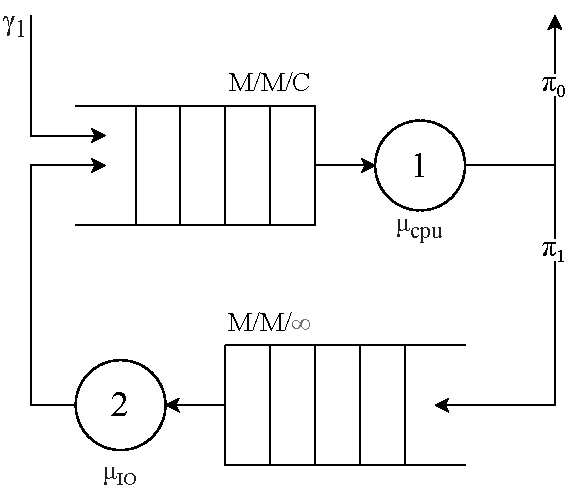
\includegraphics[width=\textwidth]{files/queue_schema.pdf}
    \end{columns}
\end{frame}

%------------------------------------------------

\begin{frame}{OMNeT++ model}
    \begin{columns}[c] % The "c" option specifies centered vertical alignment while the "t" option is used for top vertical alignment

    \column{.45\textwidth} % Left column and width
    \begin{itemize}
        \item Process generator: exponential inter-arrival time and duration
        \item Scheduler: infinite FIFO queue or priority queue (FCFS/SJF)
        \item CPU: $N$ of them (4 or 12)
    \end{itemize}

    \column{.45\textwidth} % Right column and width
    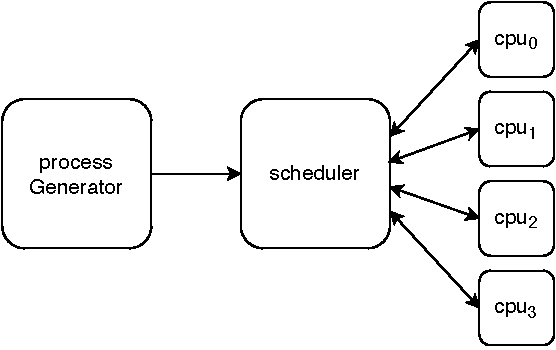
\includegraphics[width=\textwidth]{files/Computer.pdf} % oppure files/sim_schema.png
\end{columns}
    
\end{frame}

%------------------------------------------------

\begin{frame}{Warm-up and Simulation Time}
    \begin{columns}[c]
        \column{.95\textwidth}
        We used number of busy CPUs (out of $N = 4$) as metric.
    \end{columns}
    \begin{columns}[c] % The "c" option specifies centered vertical alignment while the "t" option is used for top vertical alignment
        \column{.45\textwidth} % Left column and width
        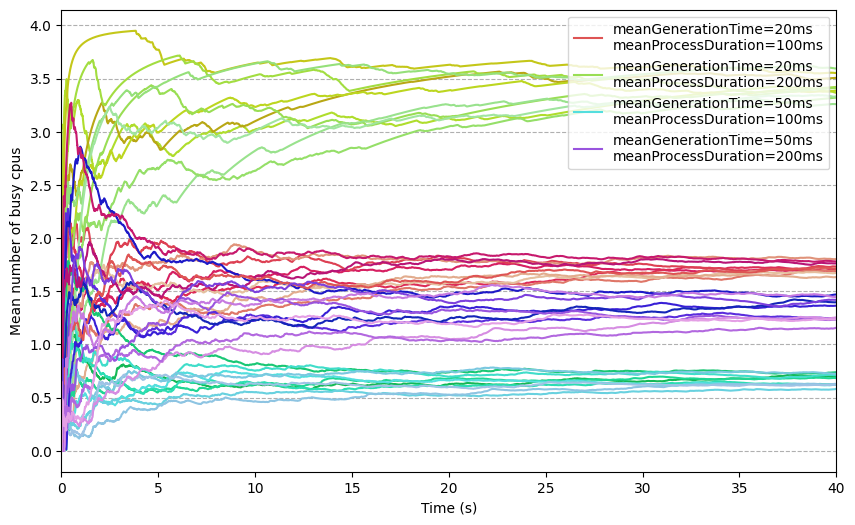
\includegraphics[width=\textwidth]{files/report_images_04/lineWarmup.png}
        \column{.45\textwidth} % Right column and width
        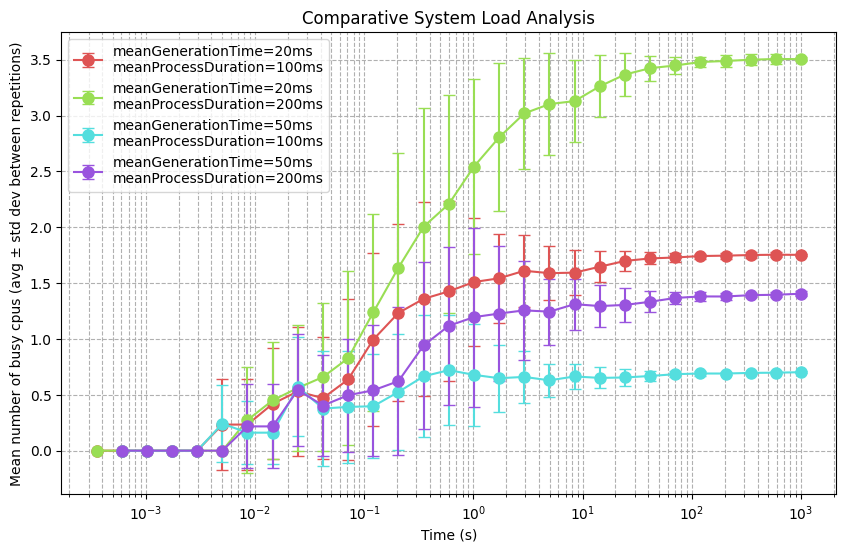
\includegraphics[width=\textwidth]{files/report_images_04/errorWarmup.png}
    \end{columns}
    \begin{columns}[c]
        \column{.6\textwidth}
        \begin{block}{}
            Chosen warm-up time: 200 s\\
            Chosen simulation time: 800 s (excluding warm-up time)
        \end{block}
        \column{.3\textwidth}
    \end{columns}
\end{frame}

%------------------------------------------------

\begin{frame}{Subsampling}
    \begin{columns}[c]
        \column{.95\textwidth}
        To test the independence of the turnaround time, we used the Ljung-Box test with a significance level of 5\%.
        When the test fails, we subsample the data.
    \end{columns}
    \begin{columns}[c]
        \column{.27\textwidth}
        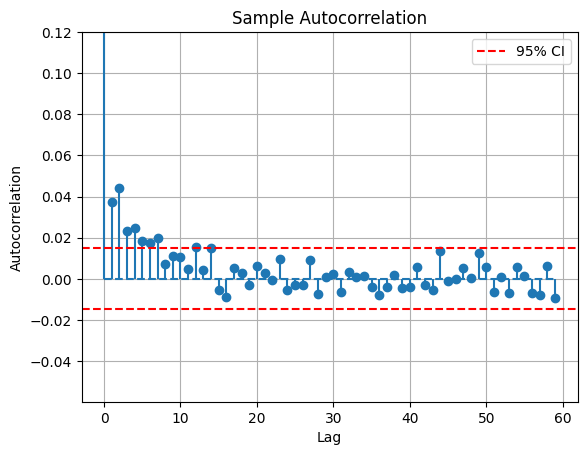
\includegraphics[width=\textwidth]{files/report_images_04/autoCor/autoCorLowUnfix.png}
        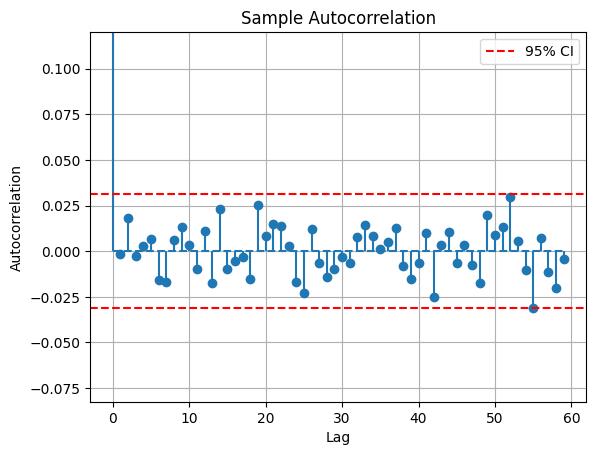
\includegraphics[width=\textwidth]{files/report_images_04/autoCor/autoCorLowFix.png}
        \column{.18\textwidth}
        $\rho=0.4$\\Q = 119\\
        \vspace{.35\textheight}
        Subsample $p=1/4$\\Q = 27
        \column{.27\textwidth}
        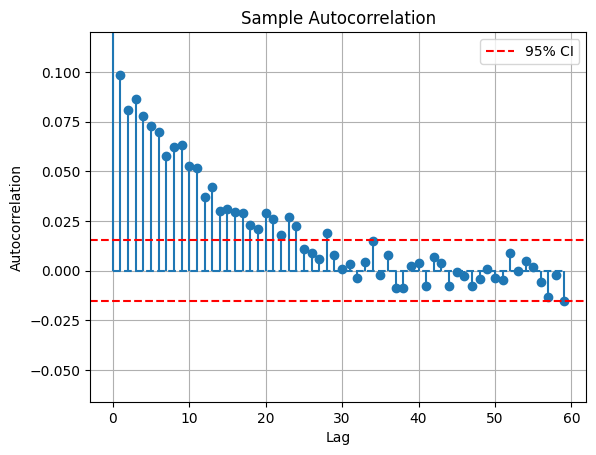
\includegraphics[width=\textwidth]{files/report_images_04/autoCor/autoCorHighUnfix.png}
        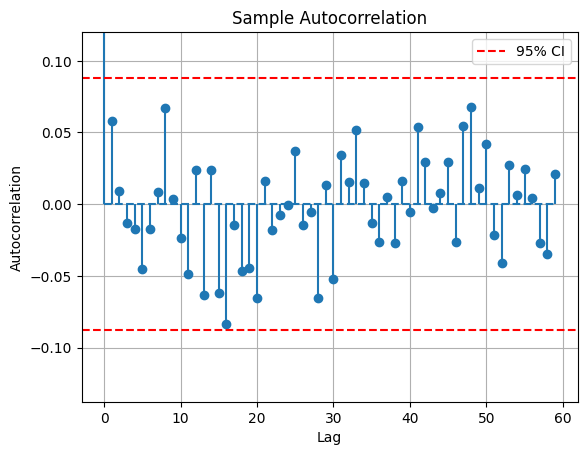
\includegraphics[width=\textwidth]{files/report_images_04/autoCor/autoCorHighFix.png}
        \column{.18\textwidth}
        $\rho=0.5$\\Q = 1333\\
        \vspace{.35\textheight}
        Subsample $p=1/16$\\Q = 22
    \end{columns}
    %\caption{Comparison of turnaround time autocorrelation with and without subsampling for different loads.}
\end{frame}

%------------------------------------------------

% TODO: togli un po' di immagini, sono troppe

\begin{frame}{FCFS Turnaround Time}
    \begin{columns}[c]
        \column{.5\textwidth}
        \includegraphics[width=\textwidth]{files/report_images_04/fcfs/turn/density.png}
        \column{.5\textwidth}
        % 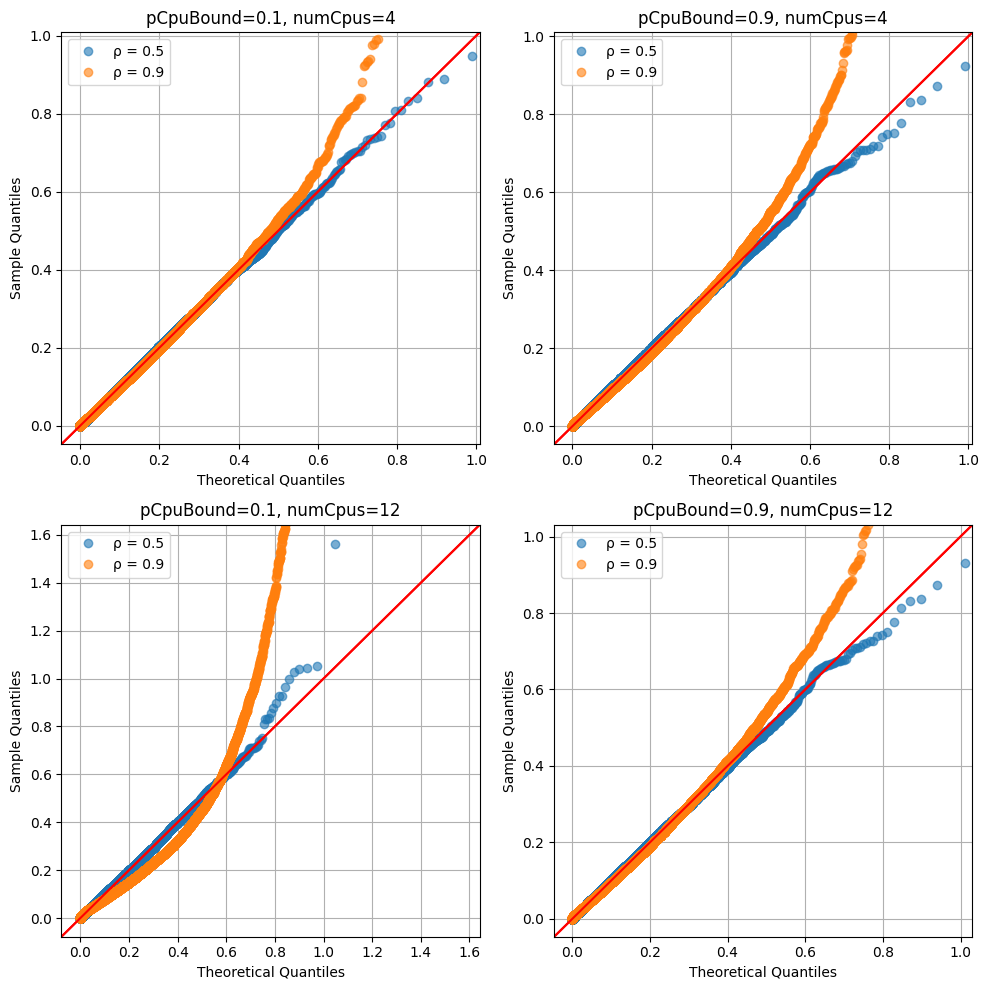
\includegraphics[width=\textwidth]{files/report_images_04/fcfs/turn/qq.png}
    \end{columns}
\end{frame}

%------------------------------------------------

\begin{frame}{FCFS Waiting Time}
    \begin{columns}[c]
        \column{.5\textwidth}
        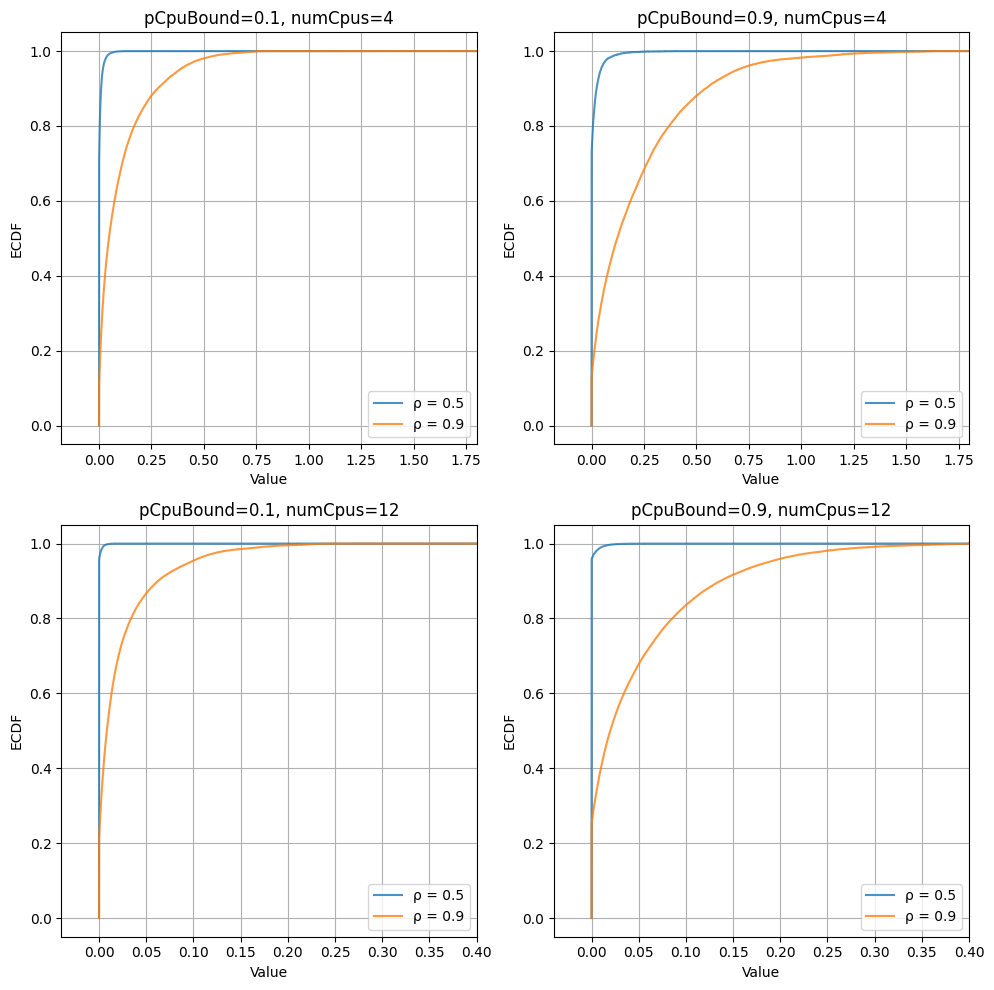
\includegraphics[width=\textwidth]{files/report_images_04/fcfs/wait/ecdf.png}
        \column{.5\textwidth}
        \includegraphics[width=\textwidth]{files/report_images_04/fcfs/wait/density.png}
    \end{columns}
\end{frame}

%------------------------------------------------

\begin{frame}{FCFS Waiting Time}
    \begin{columns}[c]
        \column{.5\textwidth}
        % 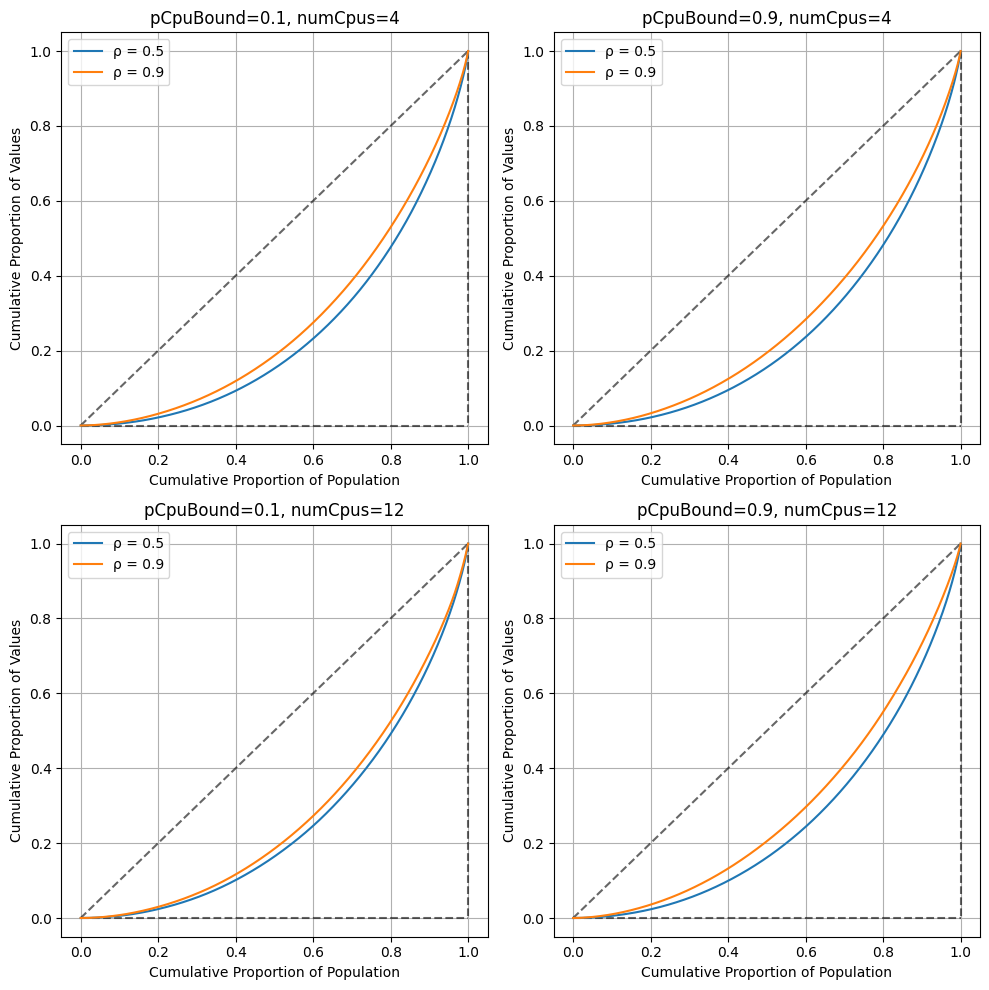
\includegraphics[width=\textwidth]{files/report_images_04/fcfs/wait/lorenz.png}
        \column{.5\textwidth}
        \includegraphics[width=\textwidth]{files/report_images_04/fcfs/wait/autocorrelation.png}
    \end{columns}
\end{frame}

%------------------------------------------------

\begin{frame}{SJF Turnaround Time}
    \begin{columns}[c]
        \column{.5\textwidth}
        \includegraphics[width=\textwidth]{files/report_images_04/sjf/turn/density.png}
        \column{.5\textwidth}
        \includegraphics[width=\textwidth]{files/report_images_04/sjf/turn/autocorrelation.png}
    \end{columns}
\end{frame}

%------------------------------------------------

\begin{frame}{SJF Waiting Time}
    \begin{columns}[c]
        \column{.5\textwidth}
        \includegraphics[width=\textwidth]{files/report_images_04/sjf/wait/density.png}
        \column{.5\textwidth}
    \end{columns}
\end{frame}

%------------------------------------------------

\begin{frame}{Conclusions}
    \begin{itemize}
        \item FCFS and SJF have similar turnaround time
        \item FCFS has higher waiting time
        \item SJF has lower autocorrelation
    \end{itemize}
\end{frame}

%----------------------------------------------------------------------------------------

\end{document}

% FCFS:
% turn around density (exp se basso, poi a cazzo) SI METTE
% turn around lorenz (lo butterei)
% turn around autocorr (alta se rho alto) (butterei visto subsampling)
% turn around qq plot vs exponential (butterei)
% 
% waiting ecdf (utile per dire che è ~= 0 per rho .5)
% waiting density (un po' a caso)
% waiting lorenz (tanto più unfair se rho basso)
% waiting autocorr (più interesting di turn around?)
% 
% SJF:
% turn around density (due exp perfetti e tanto uguali)
% turn around autocrr (scorrelati siuuu)
% turn around qq plot vs exponential
% 
% waiting ecdf (ancora più schiacciata di fcfs)
% waiting autocorr (correlati ma scendono)
% waiting lorenz (super unfair con rho basso) (lo butterei)